\documentclass[10pt,usenames,dvipsnames,svgnames,table]{beamer}
\usetheme{Warsaw}

\usepackage[english]{babel}
\usepackage[latin1]{inputenc}
\usepackage{amssymb}
\usepackage{graphicx}
\usepackage{epstopdf}
\graphicspath{ {./images/} }
\allowdisplaybreaks
\usepackage{tikz}
\setbeamertemplate{bibliography item}[text] %remove the icon
\setbeamertemplate{frametitle continuation}{}

\title[{Optimal Location of Car Wreck Adjusters}]{Optimal Location of Car Wreck Adjusters}
\subtitle{DOS Team}
\author[Luis Maltos, Roger R\'ios, Angelica Salazar, M. Gpe. Villarreal]{
  L. A. Maltos-Ortega \inst{1},
  R. Z. R\'ios-Mercado \inst{1},
  M. A. Salazar-Aguilar \inst{1}
  \and M. G. Villareal Marroquin \inst{2}}

\institute[PISIS]{
  \inst{1} Graduate Program in Systems Engineering \\
  FIME / UANL \and
  \inst{2} CIMAT Unidad Monterrey
}

\date[Oct 2015]{October 2015}

\logo{
  \makebox[0.95\paperwidht]{
    \hspace{-60pt}
    
\includegraphics[width=1.5cm,keepaspectratio]{pisis_logo}
  }
}

\AtBeginSubsection{
  \frame{\frametitle{Table of Contents}
    \tableofcontents[currentsubsection]}
}

\begin{document}
\begin{frame}
  \titlepage
\end{frame}

\begin{frame}{Contents}
  \tableofcontents
\end{frame}

%%% Introduction %%%

%En ella se deben exponer brevemente pero con absoluta claridad, 
% la novedad y actualidad del tema,
% el objeto de la investigacion,
% sus objetivos,
% la hipotesis de trabajo,
% el fundamento metodologico y
% los metodos utilizados para realizar el trabajo de investigacion.
%Es decir, que la introduccion es
% la fundamentacion cientifica de la tesis en forma resumida.

\section{Introduction}
\begin{frame}
  The aim of this work
  is to support decision making
  regarding the location and redeployment
  of insurance agents to attend car wrecks.

  The idea is to
  develop models and methods for 
  (a) improving the service 
  offered by insurance agents, 
  helping them
  arrive to the accident sites sooner,
  and 
  (b) determining the number of adjusters
  required to perform the service
  within the desired standards.

\end{frame}

\subsection{Problem}
\frame{
  The main goal is to
  determine the optimal bases (locations) 
  for placing the insurance company adjusters, 
  so as to minimize
  the average or maximum response time
  from customer calls
  when accidents occur.
  \begin{center}
    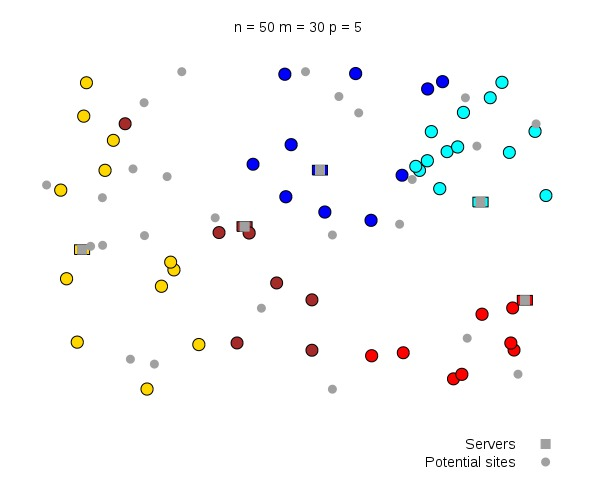
\includegraphics[scale=0.35]{SQpM_problem}
  \end{center}
}

\subsection{Motivation}
\begin{frame}
  When a car accident occurs,
  traffic congestion starts to pile up.
  This is because
  customers are not allowed
  to move their vehicles
  until the adjuster arrives.  
  The adjuster must record and determine
  the causes of the accident, 
  in order to
  move the car from the accident area
  and restore the flow.
  \begin{center}
    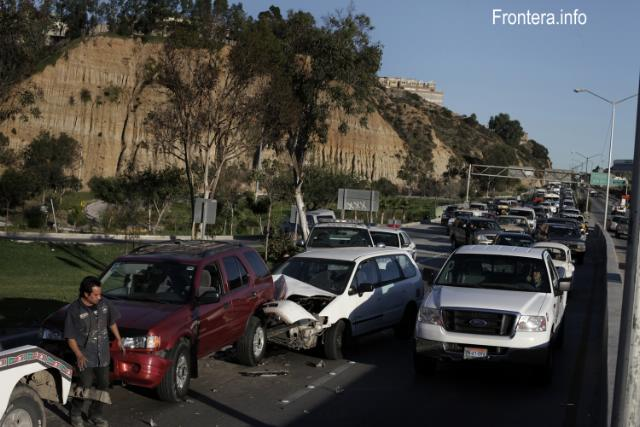
\includegraphics[scale=0.25]{389200-G}
  \end{center}
\end{frame}

% Approximating the Equilibrium Behavior of Multi-Server Loss Systems
% Jarvis - Management Sience
% 1985

\section{Approximating the Equilibrium Behavior of MSLS}
\begin{frame}
  In Jarvis \cite{jarvis1985approximating} a procedure is given for approximating the equilibrium behavior of 
  multi-server loss systems having distinguishable servers
  and multiple customers types under light to moderate traffic intensity.
\end{frame}

\subsection{Introduction}
\begin{frame}
  In an emergency service such as fire or police, 
  the servers are fire fighting units or patrol cars
  and the customers are calls for service.
  The simple Erlang loss system  is inadequate in two aspects for a detailed system analysis.
  \begin{enumerate}
  \item one often wishes to preserve the identity of service units (distinguishable servers).
  \item because of the geographic nature of these systems,
    the service time depend on both the server and the customer at least through the travel time between the pair.
  \end{enumerate}
\end{frame}

\subsection{Model assumptions, Notation, and Terminology}
\begin{frame}
  Consider a system in which:
  \begin{enumerate}
  \item Exactly one server is assigned to each customer unless all servers are busy, 
    in which case the customer is irrevocably lost of the system
  \item Servers are assigned to customers according to a fixed preference assignment rule
  \item No preemption of service is allowed
  \item Assignments are made immediately upon customer arrival
  \end{enumerate}
\end{frame}

\begin{frame}
  and we have the following parameters
  \begin{enumerate}
  \item \textit{N} distinguishable servers
  \item \textit{C} types of customers
  \item Customers of type \textit{m} arrive according to a Poisson process with rate $\lambda_{m}$
  \item $\lambda$ total arrival rate
  \item $a_{mk}$ be the \textit{k}th preferred server for customers of type \textit{m}
  \item $\tau_{im}$ the expected service time for server \textit{i} and customer of type \textit{m}
  \end{enumerate}
\end{frame}

\begin{frame}
  The performance measures for the system include 
  \begin{enumerate}
  \item $\rho_i$ the workload of server \texit{i}
  \item $f_{im}$ the probability a random customer of type \textit{m} is assigned to server \textit{i}
  \item $P_{N}$ the probability all servers are busy
  \end{enumerate}
\end{frame}

\subsection{Approximation Procedure}
\begin{frame}
  The procedure described is based on that given by Larson \cite{larson1975approximating}
  for approximating performance measures for the Hypercube model assuming exponential service times.
  Larson developed an approximation for $f_{im}$ as
  \begin{equation} \label{f_im}
    f_{im} \simeq Q(N,p,k-1)(1-\rho_{i})\prod_{l=1}^{k-1}{\rho_{a_{ml}}}
  \end{equation}
  where
  \begin{equation} \label{Q}
    Q(N,p,k)=\sum_{j=k}^{N-1}{\frac{(N-j)(N^j)(\rho^{j-k})P_0(N-k-1)!}{(j-k)!(1-P_N)^kN!(1-\rho(1-P_N))}} \\
    \hfill \mbox{for} k = 0,1,\ldots,N-1
  \end{equation}
\end{frame}

\begin{frame}
  Let $B_i$ denote the event that server \textit{i} is busy;
  and let $B_{im}$ denote the event that server \textit{i} is busy serving a customer of type \textit{m}, then
  \begin{equation} \label{rho_i}
    \rho_{i} = Pr\left[B_i\right] = \sum_{m=1}^{C}{Pr\left[B_{im}\right]} = \sum_{m=1}^{C}{\lambda_{m}f_{im}\tau_{im}}
  \end{equation}
  combine equations (\ref{f_im}) and (\ref{rho_i}) and solve for $\rho_i$ to obtain the approximation iteration
  \begin{equation}
    \rho_i\mbox{(new)}=\frac{V_i}{(1+V_i)}
  \end{equation}
  where $V_i$ is given by
  \begin{equation} \label{V_i}
    V_i = \sum_{k=1}^{N}{\sum_{m:a_{mk}=i}{\lambda_m \tau_{im} Q(N,\rho,k-1)\prod_{l=1}^{k-1}{\rho_{a_{ml}}}}}
  \end{equation}
\end{frame}

\begin{frame}
  When there is a common mean service time, the estimates for $\rho_i$ can be normalized using
  \begin{equation} \label{P_N}
    \sum_{i=1}^{N}{\rho_i} = N \rho (1 - P_{N})
  \end{equation}

  In the generalized procedure, $\tau$ can be approximated at the end of each iteration by
  \begin{equation} \label{tau}
    \tau = \sum_{m=1}^{C}{\left(\frac{\lambda_m}{\lambda}\right)\sum_{i=1}^{N}{\frac{\tau_{im}f_{im}}{(1-P_N)}}}
  \end{equation}
\end{frame}

\begin{frame}{Approximation Algorithm}{}
  {\footnotesize
    \begin{center}
      \textit{ Approximation Algorithm}
    \end{center}
    \vspace{-8pt}
    \hline \\
    \vspace{2pt}
    \textit{Given:}
    \begin{equation*}
      \lambda_m,\tau_{im},a_{mk}\mbox{  for } m = 1,\ldots,C;i=1,\ldots,N;k=1,\ldots,N \hfill
    \end{equation*}
    \textit{Initialize:}
    \begin{equation*}
      \rho_i = \sum_{m: a_{m1} = i}{\lambda_m \tau_{im}}; \; \tau = \sum_{m=1}^{C}{(\lambda_m/\lambda)\tau_{a_{m1},m}} \hfill
    \end{equation*}
    \textit{Iteration:}\\
    (1) Compute $Q(N,\rho,k)$ for $k = 1,\ldots,N-1$ where $\rho = \lambda \tau / N$ using equation (\ref{Q}). \\
    (2) For $i = 1,\ldots,N$, the new $\rho_i$ is $V_i/(1+V_i)$, where $V_i$ is given by equation (\ref{V_i}). \\
    (3) Stop if max change in $\rho_i$ is less than convergence criterion. \\
    (4) Else compute $P_N$ by equation (\ref{P_N}), $\tau$ by equation (\ref{tau}), and $f_{im}$ by equation (\ref{f_im}). \\
    (5) Return to step 1. \\
    \hline
  }
\end{frame}

\begin{frame}
  No analytic bounds on the accuracy or convergence properties of the approximation procedure have been developed.

  In regards to convergence properties,
  the numerical iteration has proved to be very stable and converges in a small number of iterations under relatively stringent conditions,
  with 4 to 6 iterations being typical for 10 servers systems.

  In comparing the accuracy of this approximation to results of the exact Hypercube model,
  Larson has found errors in server workloads to be less than 1 to 2 percent.
\end{frame}


%Emergency service systems: 
%The use of the hypercube queueing model in the solution of probabilistic location problems

\section{Hypercube queening model}
\subsection{Introduction}
\begin{frame}
  Given a system configuration, 
the hypercube model is able to evaluate a variety of performance
measures relevant for decision-making, 
either region-wide or for each server or region.

These include 
server workloads, 
mean user response times, 
fraction of dispatches of each server to each region,
among others.
\end{frame}

\begin{center}
  % Pendiente, ajustas coordenadas
  \begin{tikzpicture}
    \node[anchor=south west,inner sep=0] at (0,0) {
      %\includegraphics[width=0.9\textwidth]{tmax}
      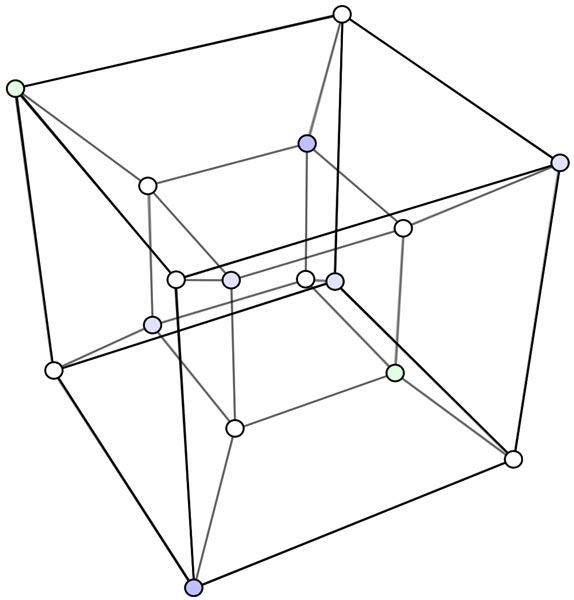
\includegraphics[scale=0.3]{hypercube}
    };
    \draw (2.5,0.1) node {\scalebox{.4}{(0,0,0,0)} };
    \draw (5.9,1.5) node {\scalebox{.4}{(0,0,0,1)} };
    \draw (2.9,1.8) node {\scalebox{.4}{(0,0,1,0)} };
    \draw (1,2.4) node {\scalebox{.4}{(0,1,0,0)} };
    \draw (2.2,3.65) node {\scalebox{.4}{(1,0,0,0)} };
  \end{tikzpicture}
\end{center}
\end{frame}

\subsection{Basic assumptions}
\begin{frame}{Geographical atoms and arrival processes}
  \begin{enumerate}
  \item The region is divided into \textit{M} geographical atoms,
    which correspond to non-overlapping areas of a city
  \item The emergency calls of each atom \textit{j} occur as a Poisson
    process, independently from the other atoms, with mean arrival rate $\lambda_j$
  \item The mean travel times $\tau_{ij}$ between atoms are known
  \end{enumerate}
\end{frame}

\begin{frame}{Servers and service processes}
  \begin{enumerate}
  \item There are \textit{N} spatially distributed servers, 
    which can service any atom
  \item Each server, when idle, stays in its base waiting for a call, 
    or moves inside a determined area
  \item The service time for a call includes the set-up time, 
    the travel time from the base until the location of the accident, 
    the on-scene time, a possibly related follow-up time, 
    and the travel time back to the base
  \item Variations in the service time that are due to variations in travel time 
    are assumed to be of second order when compared with variations of set-up, 
    on-scene and related follow-up times
  \end{enumerate}
\end{frame}

\begin{frame}{Server assignment and fixed-preference dispatching}
  \begin{enumerate}
  \item In response to each call, 
    exactly one server is dispatched from its base to the location of the accident
  \item If there are no available servers, 
    the call is either queued and serviced according to an FCFS discipline,
    or it is lost
  \item There is a list of dispatching preferences for each atom
  \end{enumerate}
\end{frame}

\subsection{Calibration process of the mean service times}
\begin{frame}
In this emergency system, 
travel times may represent a considerable part of service times. 
It may be advisable to adjust the service times by means of a calibration process,
which can be performed using a simple iterative procedure.

The procedure consists of 
verifying if there are significant differences among 
the input mean service times and the output mean service times (computed by the hypercube model). 
In this case, 
the hypercube is solved using the computed mean service times as inputs, 
until the differences among input and output values are sufficiently small
\end{frame}

\begin{frame}{}{}
  {\footnotesize
  \begin{center}
    The mean service time calibration method
  \end{center}
  \vspace{-8pt}
  \hline \\
  \vspace{2pt}
  \textit{Step 0.} The mean service time of unit \textit{i},
  $1/\mu^{i}=1/\mu_{NT}^{i}$, $i = 1,\ldots,p$ 
  ($1/\mu_{NT}^{i} = \sum_{j=1}^{n}{h_j\bar{W_{ij}}}$ 
  is the mean of non-travel time component of the service time). \\
  \textit{Step 1.} Run the Hypercube Model (using $\mu^i$) to obtain $f_{ij}$, $i = 1,\ldots,p$, $j = 1,\ldots,n$. \\
  \textit{Step 2.} $1/\hat{\mu}^{i} = \sum_{k=1}^{n}{h_{k}^{i}(\bar{W_{ik}}+(\beta_{i}/v_{i})d_{ik})}$ where $h_{k}^{i} = f_{ik}/\sum_{j=1}^{n}{f_{ij}}$ \\
  \textit{Step 3.} If $|1/\hat{\mu}^{i}-1/\mu^{i}|>\epsilon$ for at least one $i$, $i=1,\ldots,p$, set $1/\mu^{i} \equiv 1/\hat{\mu}^{i}$ and go back to \textit{Step 1.} Otherwise stop. \\
  \hline
}
\end{frame}


%%% Future Work %%

%Things to not do in your conclusion:

%   Introduce new information.
% The conclusion is for wrapping up everything you hacve done.
% It's not a place to say “oh yeah,
% and we also got result y.”
% All results should be first presented and detailed in the result section.
% Think of the conclusion as a place to reflect on what you have
% already said earlier in the paper.
%   Directly re-quote anything you’ve already written.
% I’ve seen conclusions that are almost identical
% to the abstract or a collection of sentences from throughout the paper.
% As a reader, it makes me think the author was lazy
% and could not be bothered to actually summarize their results for the paper.
% Take the time to write a proper conclusion
% so that the reader walks away with good thoughts about your work.
%   Write a conclusion longer than your introduction.
% A conclusion should be short, and to the point.
% You’ll rarely see them over 3 paragraphs,
% and three is often long.
% A lot of the time they are usually only one or two.
% Think about a conclusion as a chance to see
% how concisely you can summarize your entire research project.
% It’s your “30 second” research spiel.

\section{Future Work}
\subsection{Future Work}
\begin{frame}{Future Work}
  \begin{itemize}
  \item \textst{Design and implement heuristic methods to perform a local search}
  \item \textst{Develop a simulator to evaluate the quality of the solutions}
  \item Running pending tests
  \item Generate instances from real data
  \end{itemize}
\end{frame}


\subsection{Acknowledgements}
\begin{frame}{Acknowledgements}
\begin{itemize}
\item CONACYT (Graduate Fellowship)
\item CONACYT (grant 2011-1-166397)
\item UANL
\item FIME
\end{itemize}

\end{frame}


%%% References %%%
\subsection{References}
\begin{frame}[allowframebreaks]
  %\setbeamertemplate{bibliography item}{\insertbiblabel}
  \frametitle{References}
  {\scriptsize
    \bibliographystyle{abbrv}
    \bibliography{references}
  }
\end{frame}
\end{document}
